\documentclass[a4paper]{article}
%%%%%%%%%%%%%%%%%%%%%%%%%%%%%%%%%%%%%%%%%%%%%%%%%%%%%%%%%%%%%%%%%%%
% Packages using
%%%%%%%%%%%%%%%%%%%%%%%%%%%%%%%%%%%%%%%%%%%%%%%%%%%%%%%%%%%%%%%%%%%
\ifx\pdfoutput\undefined
	\usepackage[dvips]{graphicx}
	\DeclareGraphicsExtensions{.eps}
\else
	\usepackage[pdftex]{graphicx}
	\DeclareGraphicsExtensions{.pdf,.jpg,.png,.mps}
	\pdfcompresslevel=9
\fi
\usepackage[bookmarks=true,bookmarksnumbered=true,hypertexnames=true,breaklinks=true,colorlinks=true]{hyperref}
\usepackage{amsmath,amssymb}
\usepackage[ansinew]{inputenc}
\usepackage[english]{babel}
\usepackage{indentfirst}
\addtolength{\topmargin}{-20mm}
\addtolength{\textheight}{10mm}
%%%%%%%%%%%%%%%%%%%%%%%%%%%%%%%%%%%%%%%%%%%%%%%%%%%%%%%%%%%%%%%%%%%

\begin{document} 
	
	\title{Information Retrieval Report}
	\author{Torbj�rn Nordling, \\Eric Lee, Jacky Wu, Karthick Mani, \\Eric Chang, Dexter Cheng, Peter Cheng}  % Please add your name here
	\maketitle   
	
	\section*{Background}
	\label{Background}
	
	Whole project is seperaed to four major parts:
	\begin{enumerate}
		\item Create a data base of open access full text articles responded by team Wolverine
		\item Create a complementary XML structure for metadata that contains all information in the PDF and can be show in Utopia responded by team Eagle unit
		\item Automatic creation of metadata/markup by use of natural language processing of full text articles responded by team Union
		\item Automatic creation of links from full text articles to external sources responded by team Hanky Phanky
	\end{enumerate}
	
	%%%%%%%%%%%%%%%%%%%%%%%%%%%%%%%%%%%%%%%%%%%%%%%%%%%%%%%%%%%%%%%%%%%
% Sprint 3
% Team:
% Wolverine
% Members: 
% Eric Lee, Jacky Wu, Karthick Mani, 
% Eric Chang, Dexter Cheng, Peter Cheng
% Relative files:
% Team_Wolverine.tex, Team_Wolverine_Compile.tex, Library.bib, WolverineChart.png
% Note:    
% Do not compile this file compile Team_Wolverine_Compile.tex to get the pdf file instead.
%%%%%%%%%%%%%%%%%%%%%%%%%%%%%%%%%%%%%%%%%%%%%%%%%%%%%%%%%%%%%%%%%%%
	
\subsection*{Team Wolverine}
\label{Group}
	
Eric Lee, Jacky Wu, Karthick Mani, Eric Chang, Dexter Cheng, Peter Cheng
	
\subsection*{Create a data base of open access full text article}
\label{task1}

Goal for this subsection is to build up a database which downloads articles from open access databases using web crawler or web robot. And setting up a system that can allow the users to access the data in our database. I'd like to seperate this subsection into six features, then I'll give several suggestions based on each feature. 

\paragraph*{Feature 1 -- Database Management Systems}
\label{task1:feature6}

The relational database model was proposed by Edgar Codd in 1970, but because of the technological requirements it was not universal at that time. It was until 1980s that the first commercial relational database management systems began to appear. 
A database management system (DBMS) is a computer software application that interacts with the user, other applications, and the database itself to capture and analyze data. Well-known DBMSs include MySQL, PostgreSQL, Microsoft SQL Server, Oracle, Sybase and IBM DB2. And they can support different kinds of databases.

\subparagraph{1. Object-oriented database}
An object-oriented database (OODBMS) is a kind of database management system.\cite{WiKiauthor2013} The information in the database is represented as objects as used in object-oriented programming.
Because of the tighter integration with object-oriented language, the programmer is easier to maintain consistency with the same representation in both OODBMS and programing language.

Although relational databases which is table-oriented might be similar to object-oriented databases, But they are actually different. Object-oriented database supports objects, classes and inheritance in database schemas and query language.
There are many advantages for OODBMS compared to relational database management system(RODBMS) such as the performance, flexibility, and development cost.

And also some disadvantages, the \cite{Systems2010} have mantion 3 disadvantage for \\
OODBMS. First, because the usage is forced to be similar with object-oriented language. This make maintaining and evolving is  difficult. Second, the technic for store complex type of information take additional computational resources. Third, lack of a standard data model leads to design errors and inconsistencies.

\subparagraph{2. Relational database}
A relational database is the most popular \\
database used in the world. They can organize data into one or more tables of columns and rows, with a unique key identifying each row. Rows are also called records or tuples. Generally, each table represents one "entity type" (such as customer or product). The rows represent instances of that type of entity (such as "Lee" or "iPhone 6") and the columns representing values attributed to that instance (such as address or price).
Because of the method of the organization of data, relational database is much easier to understand and is flexible for you to manipulate the data. Besides SQL is easy in the relational database approach. For data organized in other structure the query language either becomes complex or extremely limited in its capabilities. However, once the attributes of data become more and more, you'll need a large amount of table to store your information. Therefore, the performance of relational database will decrease obviously.

\subparagraph{3. Graph database}
\label{task1:part0}
Put your article here


\paragraph*{Feature 2 --Administrator}
\label{task1:part1}

In this part, the main consideration is the relationship between user and administrator. As an administrator's point, I'd like to give the best product to the consumer. On the other hand, users want to have convenient searching engine to get in touch with the knowledge. For this purpose, I'm pressure to show two suggestions for enhancing the relationship between users and producers. First, set up a popular-word-ranking system. When I search in something I don't know its name but know it in some specific area, such as stem cell in medical area. In this moment, the popular-word-ranking system will help me searching by giving me some keywords. Then, I would be easily to use this database. Of course, the popular-word-ranking system is based on users' searches and experts'suggestions to change the key words. So, the system can be trusted. 
	
Second, build up an area in the database and let user to change the area to what they want it to be. The idea is referenced from well-known media, Wikimedia. It's so called "personalized searching". By doing this, it would help user idealize the system to what they want and suggest administrator the service which clients really want. It would lead to a win-win situation.
	
\paragraph*{Feature 3 -- Web Crawler}
\label{task1:feature2}
	
The web crawler is a algorithm that has ability to quickly and accurately process and update a very large amount of data which are constantly being updated.\cite{Liu2012} It starts with a list of URLs to visit, called the seeds. As the crawler visits these URLs, it identifies all the hyperlinks in the page and adds them to the list of URLs to visit, called the crawl frontier. URLs from the frontier are recursively visited according to a set of policies. If the crawler is performing archiving of websites it copies and saves the information as it goes. The archives are usually stored in such a way they can be viewed, read and navigated as they were on the live web, but are preserved as �snapshots'.\cite{Du2013} We need to build up a web crawler to automatically visit a list of web page. Then find out which link in the page is valuable to download it into our database. 
	
\paragraph*{Feature 4 -- User account}
\label{task1:feature3}
	
In this part, the main issue is how to create a user account that can connect between user and database. But the more important thing is to make sure database will not collapse by user who is not allowed to access to core part of database.
To protect the database system security and privilege, this study introduces two methods for user account, principle of least privilege and role-based access control respectively. The principle of least privilege, also known as the principle of minimal privilege, means giving a user account only those those privileges which are essential to that users work \cite{PrincipleLeastPrivilege}. The role-based access control is a policy neutral access control mechanism defined around privileges and roles. It can implement discretionary access control (DAC) or mandatory access control (MAC). The role-based access control is very easy to do user assignments as the components of this policy, such as role-permissions, etc. That is why it sometimes referred to as role-based security \cite{RoleBasedAccessControl}. The information and resources would not in danger due to these two methods will filter user depend on their authority and only allow the legitimate user to access.	
To protect the database system security and privilege, this study introduces two methods for user account, principle of least privilege and role-based access control respectively. The principle of least privilege, also known as the principle of minimal privilege, means giving a user account only those those privileges which are essential to that user`s work \cite{PrincipleLeastPrivilege}. The role-based access control is a policy neutral access control mechanism defined around privileges and roles. It can implement discretionary access control (DAC) or mandatory access control (MAC). The role-based access control is very easy to do user assignments as the components of this policy, such as role-permissions, etc. That is why it sometimes referred to as role-based security \cite{RoleBasedAccessControl}. The information and resources would not in danger due to these two methods will filter user depend on their authority and only allow the legitimate user to access.
	
\paragraph*{Feature 5 -- User Interface}
\label{task1:feature4}
	
Understanding the types of visualizations people create by themselves for personal use. As part of this recent direction, we have studied a large collection of whiteboards in a research institution, where people make active use of combinations of words, diagrams and various types of visuals to help them further their thought processes. Our goal is to arrive at a better understanding of the nature of visuals that are created spontaneously during brainstorming, thinking, communicating, and general problem solving on whiteboards.\cite{Blascheck2016} We use the qualitative approaches of open coding, interviewing, and affinity diagramming to explore the use of recognizable and novel visuals, and the interplay between visualization and diagrammatic elements with words, numbers and labels. We discuss the potential implications of our findings on information visualization design. Combining the advantage of visual thinking new standard of data processing, that visual nature of computers can challenge the first generation of hackers, An icon is an image, picture, or symbol representing a concept.\cite{Szpunar2010}
	
\paragraph*{Feature 6 -- Data Storage and Search Methods}
\label{task1:feature5}

The organization of data inside a database management system(DBMS) and retrieval methods is based on the database storage structure such as tables and indexes. 
There are several types of database storage structure such as XML, a textual data format. 
This advantage is self-describing and flexible in organizing data.\cite{ISI:000253400700005}Several considerations of data storage include right space allocation techniques, data compression techniques (if necessary), security and encryption and the access path to retrieve the data. 
Therefore, DBMS software provides some method to optimize and  minimum storage space of a database.



	
\begin{figure*}[h]
	\begin{center}
		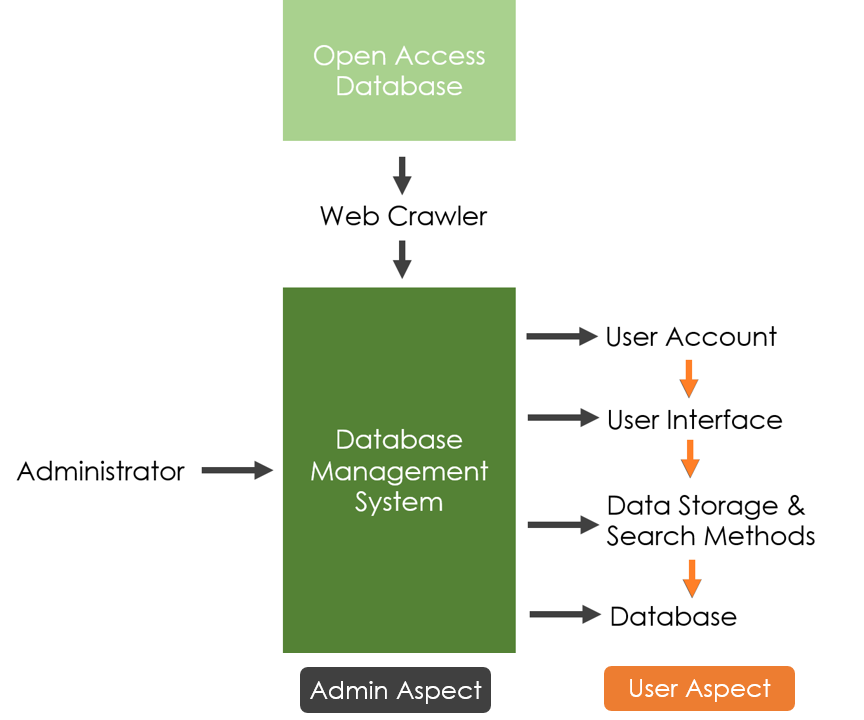
\includegraphics[scale=1.0]{WolverineChart}
	\end{center}
	\caption{Hierarchical overview}
\end{figure*}
\clearpage

	%\documentclass[a4paper]{article} % Document type

\ifx\pdfoutput\undefined
    %Use old Latex if PDFLatex does not work
   \usepackage[dvips]{graphicx}% To get graphics working
   \DeclareGraphicsExtensions{.eps} % Encapsulated PostScript
 \else
    %Use PDFLatex
   \usepackage[pdftex]{graphicx}% To get graphics working
   \DeclareGraphicsExtensions{.pdf,.jpg,.png,.mps} % Portable Document Format, Joint Photographic Experts Group, Portable Network Graphics, MetaPost
   \pdfcompresslevel=9
\fi

\usepackage{amsmath,amssymb}   % Contains mathematical symbols
\usepackage[ansinew]{inputenc} % Input encoding, identical to Windows 1252
\usepackage[english]{babel}    % Language
\usepackage[round,authoryear]{natbib}  %Nice author (year) citations
%\usepackage[square,numbers]{natbib}     %Nice numbered citations
%\bibliographystyle{unsrtnat}           %Unsorted bibliography
\bibliographystyle{plainnat}            %Sorted bibliography

\addtolength{\topmargin}{-20mm}% Removes 30mm from the top margin
\addtolength{\textheight}{10mm}% Adds it to the text height


\begin{document}               % Begins the document

\title{Automatic creation of metadata/markup by use of natural language processing of full text articles}
\author{First name Last name \\ student number \\ email} 
%\date{2010-10-10}             % If you want to set the date yourself.

\maketitle                     % Generates the title

\section*{overview}
\label{sec:prob}

We�re producing a program which automatically generate metadata such as authors� name, date of publishing, name of articles� and more importantly auto-abstract for full text articles
We are interested in features for either more convenient use of the program or improving precise data generation
There are 5 related problems.\\
\includegraphics[scale=0.3]{../Picture1}\\
Figure 1. Overview of metadata creation process.\\

\section*{Problem 1}
\label{sec:prob}
When  users  search  with  a  sentence,  how  do  the  program  understand  the  certain  input  of  text?  

\section*{Method 1}
\label{sec:meth}

Building  a  natural  language  understanding  (NLU)  system.
\section*{Solution 1}
\label{sec:solu}

Use  a  set  of  possible  yes-no  questions  that  can  be  applied  to  data  items,  then  follow  a  rule  for selecting  the  best  question  at  any  node  on  the  basis  of training  data,  which  has  a  method  for  pruning trees to prevent over-training.


\section*{Problem 2}
\label{sec:prob}
When users search Turkey, the results could be a country or an animal. Sometimes, the results are totally unrelated. 

\section*{Method 2}
\label{sec:meth}
categorize the results based on different subjects or genres

\section*{Solution 2}
\label{sec:solu}

It�s significantly crucial for search engine to understand what users want by name recognition in natural language processing.  Digital libraries and web resources have limited metadata, augmenting them with meaningful, stable and desired categories. Information can enable better overviews and support user exploration.  

\section*{Problem 3}
\label{sec:prob}
Word sense disambiguation

\section*{Method 3}
\label{sec:meth}
Word sense disambiguation is an important step in natural language processing. This is the step where words with different meaning will be listed in different category (Abualhaija and Zimmermann, 2016). WSD has been done with three main approaches: supervised disambiguation (Abualhaija and Zimmermann, 2016), semi-supervised approach (Ben Aouicha et al., 2016), and more recently unsupervised approach (Yoon et al., 2006). Research for unsupervised approach has been developed quickly and application of this approach has been found in WSD for not-so-popular language such as Korean. 

\section*{Solution 3}
\label{sec:solu}
The project team has decided to pursuit the unsupervised approach. Implementation will be made in term of symnonym grouping (Navigli, 2009) and context clustering (Wang et al., 2009).

\section*{Problem 4}
\label{sec:prob}
The readers do not know what the connected words meaning

\section*{Method 4}
\label{sec:meth}
Compute and Analyze in natural language processing

\section*{Solution 4}
\label{sec:solu}
I suggest we should use the Python language to complete this task. 
It can easily conpute and analyze the words in the articles.
Phthon can compute and analyze by separating the connected words.
The readers can know what do the words mean when they are reading the articles .



\section*{Problem 5}
\label{sec:prob}
Natural language processing help us extract the important information from the full text article.
How could we make it more efficiently and precisely?


\section*{Method 5 test}
\label{sec:meth}
Query reduction to single sub-query


\section*{Solution 5}
\label{sec:solu}
 The performance of the machine is better in the short query rather than long query. Thus, it is an important issue to reduce the query to many sub-query.  The first is extracting the single sub-query by the existing features. Then, We combine these features to the reduction�s technique. We could find that it is more efficient than just analyze the original query. 



\section*{Reference}
\label{sec:refe}
[1].Jin 2008, Effectiveness Web Search Results for Genre and Sentiment Classification
\\\
[2].Bill 2006, Categorizing Web Search Results into Meaningful and Stable Categories Using Fast-Feature Techniques
\\\
[3].Weiscbedel 2006 White Paper on Natural Language Processing
\\\
[4].Collins 2011 Natural Language Processing Machine Learning Research
\\\
[5].Manish Gupta 2015, Information Retrieval with Verbose Queries, Foundations and Trends in Information Retrieval
\\\
[6].Julia Hirschberg 2015, Advances in natural language processing, Science
\\\
[7].Shapiro1982, A knowledge engineering approach to natural language understanding 
\\\
[8].Kuhn1995, The Application of Semantic Classification Trees to Natural Language Understanding
\\\
[9].Abualhaija, S.and Zimmermann, K.-H. 2016. D-Bees: A novel method inspired by bee colony optimization for solving word sense disambiguation. Swarm and Evolutionary Computation, 27, 188-195.
\\\
[10]. Ben Aouicha, M., Hadj Taieb, M. A.and Ezzeddine, M. 2016. Derivation of �is a� taxonomy from Wikipedia Category Graph. Engineering Applications of Artificial Intelligence, 50, 265-286.
\\\
[11]. Navigli, R. 2009. Word sense disambiguation: A survey. ACM Computing Surveys (CSUR), 41, 10. 
\\\
[12]. Wang, H., Missura, O., G�rtner, T.and Wrobel, S. 2009. Context-based clustering of image search results. In: KI 2009: Advances in Artificial Intelligence. Springer.
\\\
[13]. Yoon, Y., Seon, C.-N., Lee, S.and Seo, J. 2006. Unsupervised word sense disambiguation for Korean through the acyclic weighted digraph using corpus and dictionary. Information Processing and Management, 42, 710-722.
\\\


\end{document}      % End of the document
 % Change it to your .tex filename
	%\documentclass[a4paper]{article} % Document type

\ifx\pdfoutput\undefined
    %Use old Latex if PDFLatex does not work
   \usepackage[dvips]{graphicx}% To get graphics working
   \DeclareGraphicsExtensions{.eps} % Encapsulated PostScript
 \else
    %Use PDFLatex
   \usepackage[pdftex]{graphicx}% To get graphics working
   \DeclareGraphicsExtensions{.pdf,.jpg,.png,.mps} % Portable Document Format, Joint Photographic Experts Group, Portable Network Graphics, MetaPost
   \pdfcompresslevel=9
\fi

\usepackage{amsmath,amssymb}   % Contains mathematical symbols
\usepackage[ansinew]{inputenc} % Input encoding, identical to Windows 1252
\usepackage[english]{babel}    % Language
\usepackage[round,authoryear]{natbib}  %Nice author (year) citations
%\usepackage[square,numbers]{natbib}     %Nice numbered citations
%\bibliographystyle{unsrtnat}           %Unsorted bibliography
\bibliographystyle{plainnat}            %Sorted bibliography

\addtolength{\topmargin}{-20mm}% Removes 30mm from the top margin
\addtolength{\textheight}{10mm}% Adds it to the text height


\begin{document}               % Begins the document

\title{Structure of XML Metadata}
\author{EagleUnit \\ (I-Chieh, Chinweze, Henry, Ray, Jones, Piyarul)} 
%\date{2010-10-10}             % If you want to set the date yourself.

\maketitle                     % Generates the title




%%%%%%%%%%%%%%%%%%%%%%%%%%%%%%%%%%%%%%%%%%%%%%%%%%%%%%%%%%%%%%%%%%%%%%%%%%%%%%%%%%%
% Instructions regarding the report
%%%%%%%%%%%%%%%%%%%%%%%%%%%%%%%%%%%%%%%%%%%%%%%%%%%%%%%%%%%%%%%%%%%%%%%%%%%%%%%%%%%

\section{XML metadata structure}
\label{sec:abs}


Our responsipility is to construct an XML metadata structure.


%%%%%%%%%%%%%%%%%%%%%%%%%%%%%%%%%%%%%%%%%%%%%%%%%%%%%%%%%%%%%%%%%%%%%%%%%%%%%%%%%%%
% 1. Different standards of metadata
%%%%%%%%%%%%%%%%%%%%%%%%%%%%%%%%%%%%%%%%%%%%%%%%%%%%%%%%%%%%%%%%%%%%%%%%%%%%%%%%%%%

\subsubsection*{1. Different standards of metadata}
\label{sec:mets}
There's many different standards existing to describe the metadata in different fields and applications. We list 5 of them and give a brief introduction to each one.

\begin{enumerate}
	\item IAFA/Whois++ Templates\\
	Internet Anonymous Ftp Archive (IAFA) templates were designed to facilitate effective access to ftp (file transfer protocol) archives by means of describing the contents and services available from the archive.	
	
	\item MARC\\
	MARC was a means to allow the exchange of catalogue records between co-operating libraries, it was a format for national bibliographies to use for printed bibliographic records, and it was used by bibliographic agencies for their supply of records to libraries.
	
	\item Text Encoding Initiative (TEI)\\
	It describes the goal of the project as "to define a set of generic guidelines for the representation of textual materials in electronic form, in such a way as to enable researchers in any discipline to interchange and re-use resources, independently of software, hardware, and application area.�	
	
	\item Dublin Core\\
	The Dublin Core workshop recognised that widespread indexing and bibliographic control of Internet resources depends on the existence of a simple record to describe networked resources. The objective was to define a simple set of data elements so that authors and publishers of Internet documents could create their own metadata records in a distributed way.
	
	\item IEEE Learning Object Metadata (LOM)\\
	The LOM data schema specifies which characteristics of a learning object should be described and what vocabularies may be used for these descriptions; it also defines how this data model can be amended by additions or constraints.	
\end{enumerate}

More detailed introduction could be found in {\bf\cite{1:1:1}} and {\bf\cite{Rachel:2009:reviewofmetadataformats}}.

%%%%%%%%%%%%%%%%%%%%%%%%%%%%%%%%%%%%%%%%%%%%%%%%%%%%%%%%%%%%%%%%%%%%%%%%%%%%%%%%%%%
% 2. Necessary elements of XML metadata
%%%%%%%%%%%%%%%%%%%%%%%%%%%%%%%%%%%%%%%%%%%%%%%%%%%%%%%%%%%%%%%%%%%%%%%%%%%%%%%%%%%

\subsubsection*{2. Necessary elements of XML metadata with DTD}
\label{sec:mets}
{\bf\cite{Ruey-Shun:2003:DevelopinganXMLframeworkformetadatasystem}} suggest that an XML metadata discribed according the DTD include three necessary elements:
\begin{enumerate}
	\item Structure\\
	The major execution ability of structure includes parser for well-formed XML and
	valid DTD structure, authoring tool for editing.
	
	\item Depth\\
	Basically, there are two sorts of fields: Fixed-length fields and variable fields.
	Fixed-length fields are general types and character-indication types Sub-field, whether
	fixed-length fields or variable fields, might contain both fixed-length fields and
	variable fields. According to the reason above, the process ability of the system has to
	cover the situation
	
	\item Scope\\
	The connections must involve simple object, time, space, people, and event. 
\end{enumerate}
%%%%%%%%%%%%%%%%%%%%%%%%%%%%%%%%%%%%%%%%%%%%%%%%%%%%%%%%%%%%%%%%%%%%%%%%%%%%%%%%%%%
% 3. Other apllications
%%%%%%%%%%%%%%%%%%%%%%%%%%%%%%%%%%%%%%%%%%%%%%%%%%%%%%%%%%%%%%%%%%%%%%%%%%%%%%%%%%%

\subsubsection*{3. Other apllications of XML metadata}
Here's a few of useful tools and applications for XML metadata:
\begin{enumerate}
\item METS:\\
METS is an XML document format intended for the encoding of complex objects within digital libraries. It provides the means to record all of the descriptive, administrative, structural and behavioral metadata needed to manage and provide access to complex digital content (McDonough2006). METS provides a method for aggregating all the metadata that can be used with a digital object. ({\bf \cite{Sharon Cheslow:2014:METSForTheCulturalHeritageCommunity}})

\item PREMIS:\\
PREservation Metadata: Implementation Strategies (PREMIS) {\bf(wiki)} is an administrative metadata schema used for the preservation of digital resources ({\bf \cite{Sharon Cheslow:2014:METSForTheCulturalHeritageCommunity}}). With the rapid changes in technology, digital objects including its metadata a bound to go obsolete at some time in the future. PREMIS was created to set standards that will ensure long term usability of digital resources. 

\item MODS:\\
Metadata Object and Description Schema (MODS) is a standard for encoding metadata of digital objects using XML. MODS among XML base metadata standards has remain the most descriptive and has high level compatibility with MARC ({\bf \cite{Rebecca Guenther:2003:NewMetadataStandardsforDigitalResources}}).

\end{enumerate}




%%%%%%%%%%%%%%%%%%%%%%%%%%%%%%%%%%%%%%%%%%%%%%%%%%%%%%%%%%%%%%%%%%%%%%%%%%%%%%%%%%%
% The bibliography
%%%%%%%%%%%%%%%%%%%%%%%%%%%%%%%%%%%%%%%%%%%%%%%%%%%%%%%%%%%%%%%%%%%%%%%%%%%%%%%%%%%
%\bibliography{Bibliography_template} %Read the bibliography from a separate file

\begin{thebibliography}{99}
\bibitem[Barker(2010)]{1:1:1}
Phil Barker.
\newblock \emph{Metadata for Learning Materials: an Overview of Existing Standards and Current Developments}.
\newblock Technology, Instruction, Cognition and Learning vol 7 (3-4) 2010
\newblock http://www.oldcitypublishing.com/TICL/TICLcontents/TICLv7n3-4contents.html


\bibitem[Rachel Heery.(2009)]{Rachel:2009:reviewofmetadataformats}
Rachel Heery.
\newblock \emph{Review of Metadata Formats}.
\newblock "Review of metadata formats", Program, Vol. 30 Iss 4 pp. 345 - 373,1996
\newblock http://dx.doi.org/10.1108/eb047236

\bibitem[Ruey-Shun Chen(2003)]{Ruey-Shun:2003:DevelopinganXMLframeworkformetadatasystem}
Ruey-Shun Chen.
\newblock \emph{Developing an XML framework for metadata system}.
\newblock ISICT '03 Proceedings of the 1st international symposium on Information and communication technologies
\newblock http://dl.acm.org/citation.cfm?id=963653

\bibitem[Sharon Cheslow(2014)]{Sharon Cheslow:2014:METSForTheCulturalHeritageCommunity}
Sharon Cheslow.
\newblock \emph{METS For The Cultural Heritage Community: A	Literature Review}.
\newblock Library Philosophy and Practice (e-journal). Paper 1162.
\newblock http://digitalcommons.unl.edu/libphilprac/1162/

\bibitem[Rebecca Guenther(2003)]{Rebecca Guenther:2003:NewMetadataStandardsforDigitalResources}
Rebecca Guenther.
\newblock \emph{New Metadata Standards for Digital Resources: MODS and METS}.
\newblock Portal: Libraries and the Academy, Johns Hopkins University Press (2003)
\newblock http://onlinelibrary.wiley.com/doi/10.1002/bult.268/pdf

\end{thebibliography}


%%%%%%%%%%%%%%%%%%%%%%%%%%%%%%%%%%%%%%%%%%%%%%%%%%%%%%%%%%%%%%%%%%%%%%%%%%%%%%%%%%%
% figures
%%%%%%%%%%%%%%%%%%%%%%%%%%%%%%%%%%%%%%%%%%%%%%%%%%%%%%%%%%%%%%%%%%%%%%%%%%%%%%%%%%%
\clearpage % Ends the current page and causes all figures and tables to be printed

\begin{figure*}[p] % The * makes the figure span both columns, p places the figure on a float page
	\begin{center}
		\includegraphics[scale=1.0]{hw3.pdf}
	\end{center}
	\caption{hierarchical overview of the methods/solutions}
	\label{fig:hw3}
\end{figure*}


\end{document}      % End of the document


%tast

 % Change it to your .tex filename
	
	%%%%%%%%%%%%%%%%%%%%%%%%%%%%%%%%%%%%%%%%%%%%%%%%%%%%%%%%%%%%%%%%%%%
	% References
	%
	% I'm using Mendeley Desktop with library.bib
	%%%%%%%%%%%%%%%%%%%%%%%%%%%%%%%%%%%%%%%%%%%%%%%%%%%%%%%%%%%%%%%%%%%		
	\bibliographystyle{plain}
	\bibliography{library}	
	\clearpage 
\end{document}  
